\documentclass[12pt]{article}

% Packages
\usepackage[
  paperwidth=8.5in,
  paperheight=11in,
  margin=0.5in
]{geometry}
\usepackage{amsmath, amssymb}
\usepackage{booktabs}
\usepackage{tabularx}
\usepackage{graphicx}


\newcommand{\tacred}{FS-TACRED}
\newcommand{\qwensmall}{Qwen3-4B}
\newcommand{\gemmasmall}{Gemma3-4B}

\begin{document}

\section{Update on Prompt Optimization}

Based on our experiments so far, we observe that using feedback from both correct predictions and mistakes generally improves validation performance. However, the best-performing approach to date is surprisingly simple: optimizing the prompt without providing any feedback, i.e., asking an LLM to improve the prompt without showing any examples.

We are not yet confident that this approach is optimal. Further experiments are needed, especially since our task is a binary classification setting where the LLM outputs only \texttt{yes/no} without any reasoning.

\section{Motivation}

After reviewing several related works, it appears that the strongest methods combine multiple optimization components rather than relying on a single strategy. This motivates exploring more structured and hybrid approaches to prompt optimization.

\section{My core ideas}

\begin{enumerate}
    \item \textbf{Mutation with Prompt Traces.}  
    During mutation, we provide traces of prompt changes from parent prompts. This helps identify which changes improved validation performance and guides future mutations.

    \item \textbf{Complementary Prompt Crossover.}  
    For a sampled prompt $X$, instead of random crossover, we select a complementary prompt $Y$ that performs well on cases where $X$ performs poorly, and perform crossover between $X$ and $Y$.
\end{enumerate}

\section{Additional Ideas}

\begin{itemize}
    \item \textbf{Grouped Error Feedback.}  
    Inspired by \cite{errortaxonomyguidedpromptoptimization}, errors can be grouped into categories and provided as batch feedback, similar to batch updates in backpropagation.

    \item \textbf{Instruction + Example Optimization.}  
    As shown in \cite{teach_better_or_show_smarter}, optimizing examples using a simple instruction can outperform instruction-only optimization. Example optimization selects the best $K$ labeled relation--query instances from a pool. Combining instruction and example optimization yields the most robust performance.

    \item \textbf{MCTS-based Search.}  
    Use Monte Carlo Tree Search to balance exploration and exploitation during prompt optimization.
\end{itemize}

\section{Framework Overview}

Figure~\ref{fig:overview} presents the overall framework. Starting from an initial prompt, we first apply instruction optimization, followed by example optimization.

Figure~\ref{fig:mutation} illustrates the mutation strategy, which includes mutation without feedback, mutation with prompt traces, and mutation with explicit feedback.

Figure~\ref{fig:crossover} shows the crossover strategy, where prompts are combined either randomly or using complementary prompt selection.

\begin{figure}[ht]
    \centering
    
\includegraphics[width=0.8\linewidth]{figures/overview.pdf}
    \caption{Overview of the approach. Given an initial prompt, we will first to Instruction Optimization followed by Example Optimization.}
    \label{fig:overview}
\end{figure}

\begin{figure}[ht]
    \centering
    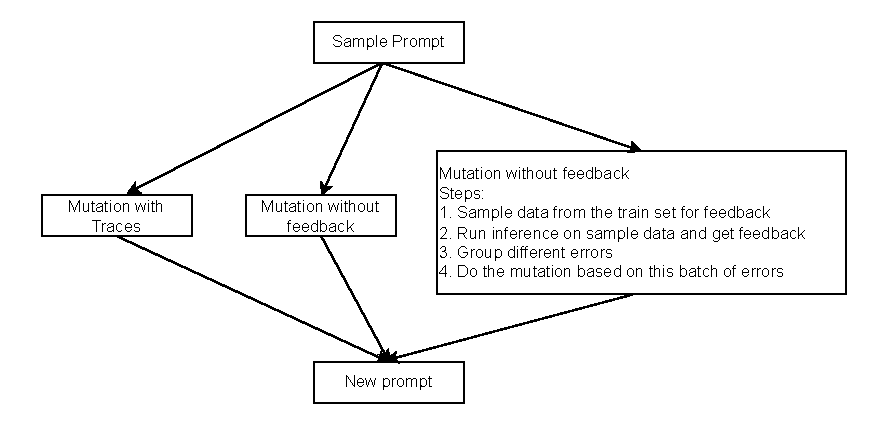
\includegraphics[width=0.8\linewidth]{figures/mutation.pdf}
    \caption{This shows the mutation approach. After we sample the prompt, we have three options to mutate this prompt: Mutate without feedback, Mutate with traces, and Mutate with feedback.}
    \label{fig:mutation}
\end{figure}

\begin{figure}[ht]
    \centering
    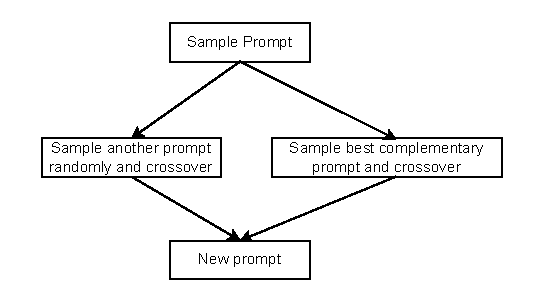
\includegraphics[width=0.8\linewidth]{figures/crossover.pdf}
    \caption{This shows the crossover approach. After we sample the prompt, do crossover with another prompt (selected randomly  or select best complimentary prompt).}
    \label{fig:crossover}
\end{figure}


\bibliographystyle{plain}  
\bibliography{custom}    

\end{document}
